\ifdefined\isdraft
   \documentclass[25pt, landscape, draft]{foils}
\else
   \documentclass[25pt, landscape, final]{foils}
\fi

\usepackage{geometry}
\usepackage{graphicx}
\usepackage[usenames,dvipsnames,svgnames]{xcolor}
\usepackage{xspace}
\usepackage{amsmath,amssymb,amsfonts} % Typical maths resource packages
\usepackage{pifont}
\usepackage{hyperref}
\usepackage{authblk}
\usepackage{pstricks}
\usepackage{pst-node}
\usepackage{booktabs}

\hypersetup{colorlinks=true, urlcolor=blue, urlbordercolor=blue,
   pdfauthor={Dmitri Smirnov <d.s@plexoos.com>}
}
% Overrides border style set with colorlinks=true. Hyperlink border style will
% be underline of width 1pt
\makeatletter
\Hy@AtBeginDocument{ \def\@pdfborder{0 0 1} \def\@pdfborderstyle{/S/U/W 1} }
\makeatother

% Requires \documentclass{foils} in the preamble
\newcommand{\myfoilhead}[2]{\foilhead[#1]{\textcolor{blueDark}{\boldmath #2}}}

% Basic commonly used commands
\renewcommand\labelitemi{\textcolor{redDark}{$\bullet$}}
\renewcommand\labelitemii{\textcolor{greenDark}{$\bullet$}}
\renewcommand\labelitemiii{\textcolor{blueDark}{$\bullet$}}

\newcommand\arabicitemii{\textcolor{greenDark}{\textbf{\arabic{listcounter}.}}}

% Requires color package
% \usepackage{color}

\definecolor{redDark}{rgb}{0.8,0,0}
\definecolor{blueDark}{rgb}{0,0,0.5}
\definecolor{blueLight}{rgb}{0.5, 0.4, 1.0}
\definecolor{blue1}{rgb}{0.8, 0.8, 1.0}
\definecolor{greenDark}{rgb}{0, .5, 0}
\definecolor{greenDark2}{rgb}{0, .4, 0}
\definecolor{greenLight}{rgb}{.8, 1.0, .8}
\definecolor{yellowDark}{rgb}{.6, .6, 0}
\definecolor{black}{rgb}{0, 0, 0}
\definecolor{yellow}{rgb}{1.0, 1.0, 0.0}
\definecolor{bgColor}{rgb}{1,1,1}
\definecolor{pink}{rgb}{1.0,0.9,0.9}
\definecolor{greyLight}{rgb}{0.8,0.8,0.8}
\definecolor{greyDark}{rgb}{0.4,0.4,0.4}


\AtBeginDocument{\color{blueDark}}

% The chosen paper size has aspect ratio of 1.6. It is a compramize between the
% varios standard paper sizes and the typical screen/projector aspect ratio of
% 16:9
\geometry{paperwidth=320mm, paperheight=200mm, includeall=true,
          centering=true, nomarginpar, headsep=0mm, headheight=0mm,
          tmargin=1mm, bmargin=1mm, lmargin=1mm, rmargin=1mm}


\newcommand{\StMuTrack}{\texttt{StMuTrack}\xspace}
\newcommand{\StTrack}{\texttt{StTrack}\xspace}
\newcommand{\Sti}{\texttt{Sti}\xspace}
\newcommand{\MinuitVF}{\texttt{MinutVF}\xspace}
\newcommand{\PPV}{\texttt{PPV}\xspace}
\newcommand{\muDST}{\texttt{muDST}\xspace}

% Symbols from pifont package
\newcommand{\cmark}{\textcolor{greenDark}{\ding{51}}}%
\newcommand{\xmark}{\textcolor{redDark}{\ding{55}}}%


\MyLogo{}
\leftheader{}
\rightheader{\footnotesize \thepage}
\rightfooter{}
\Restriction{}

\setlength{\unitlength}{0.02\textwidth}
\psset{unit=\unitlength}
\psset{framearc=.1,fillcolor=blueDark!10,linecolor=blueDark,linewidth=0.1,fillstyle=solid,arrowscale=3}


\title{\vspace{20mm} \Large Vertex Reconstruction at STAR\\[3mm] with \muDST Data Format}

\author{\quad\\[3mm]
Dmitri~Smirnov}

\affil{BNL}

\date{\small February 22, 2017}



%===============================================================================
\begin{document}

\maketitle
\addtocounter{page}{1}

\small



%===============================================================================
\myfoilhead{-30mm}{Motivation}
%{{{

\noindent
\begin{pspicture}(0,0)(\textwidth,\textheight)



\rput(0.50\textwidth,0.45\textheight) {%
\begin{minipage}{0.95\textwidth}

\raggedright

\begin{list}{\labelitemi}{\setlength{\itemsep}{0mm}
                          \setlength{\topsep}{0mm}}

   \item Two main vertex finders \MinuitVF and \PPV used for heavy-ion and
      proton-proton data respectively

   \begin{list}{\labelitemii}{\setlength{\itemsep}{3mm}
                              \setlength{\topsep}{0mm}}

      \item Classic vertex reconstruction algorithms with track pre-selection,
         seeding, fitting, and ranking stages

   \end{list}

   \item Vertex reconstruction at STAR is an integral part of full event
   reconstruction

   \begin{list}{\labelitemii}{\setlength{\itemsep}{3mm}
                              \setlength{\topsep}{0mm}}

      \item Event reconstruction runs over raw data (.daq) files with complete event information

      \item Tracking algorithm (e.g. \Sti) reconstructs global tracks, i.e.\\
      provides helix parametrization in Point of Closest Approach to $(x,y) = (0,0)$\\
      (track's DCA state) $\Longrightarrow$

      \item Vertex finder reconstructs vertices using the DCAs $\Longrightarrow$

      \item Tracking algorithm assigns primary tracks to found vertices

   \end{list}

\end{list}

\end{minipage}
}



%\psgrid[gridlabels=0.7,subgriddiv=0, griddots=3](1,-1)(0,-3)(\textwidth,\textheight)

\end{pspicture}
%}}}



%===============================================================================
\myfoilhead{-30mm}{Proposal to Use \muDST}
%{{{

\noindent
\begin{pspicture}(0,0)(\textwidth,\textheight)



\rput(0.50\textwidth,0.45\textheight) {%
\begin{minipage}{0.95\textwidth}

\raggedright

\begin{list}{\labelitemi}{\setlength{\itemsep}{0mm}
                          \setlength{\topsep}{0mm}}

   \item Run vertex finders over \muDST trees with limited information

   \begin{list}{\labelitemii}{\setlength{\itemsep}{6mm}
                              \setlength{\topsep}{0mm}}

      \item Track information is available at DCA for global tracks in \StMuTrack\\[3mm]

      $\Longrightarrow$ Can reuse existing code

      \item Save time by reconstructing tracks once\\[3mm]

      $\Longrightarrow$ Faster feedback when running as an afterburner for
      tuning, studying, or optimization purposes

      \item Track hits are not available in \muDST trees\\[3mm]

      $\Longrightarrow$ Cannot re-fit tracks without hits as in default reconstruction

   \end{list}

\end{list}

\end{minipage}
}



%\psgrid[gridlabels=0.7,subgriddiv=0, griddots=3](1,-1)(0,-3)(\textwidth,\textheight)

\end{pspicture}
%}}}



%===============================================================================
\myfoilhead{-30mm}{Source Code}
%{{{

\noindent
\begin{pspicture}(0,0)(\textwidth,\textheight)


\rput[lt](0.5\textwidth, 0.9\textheight){ 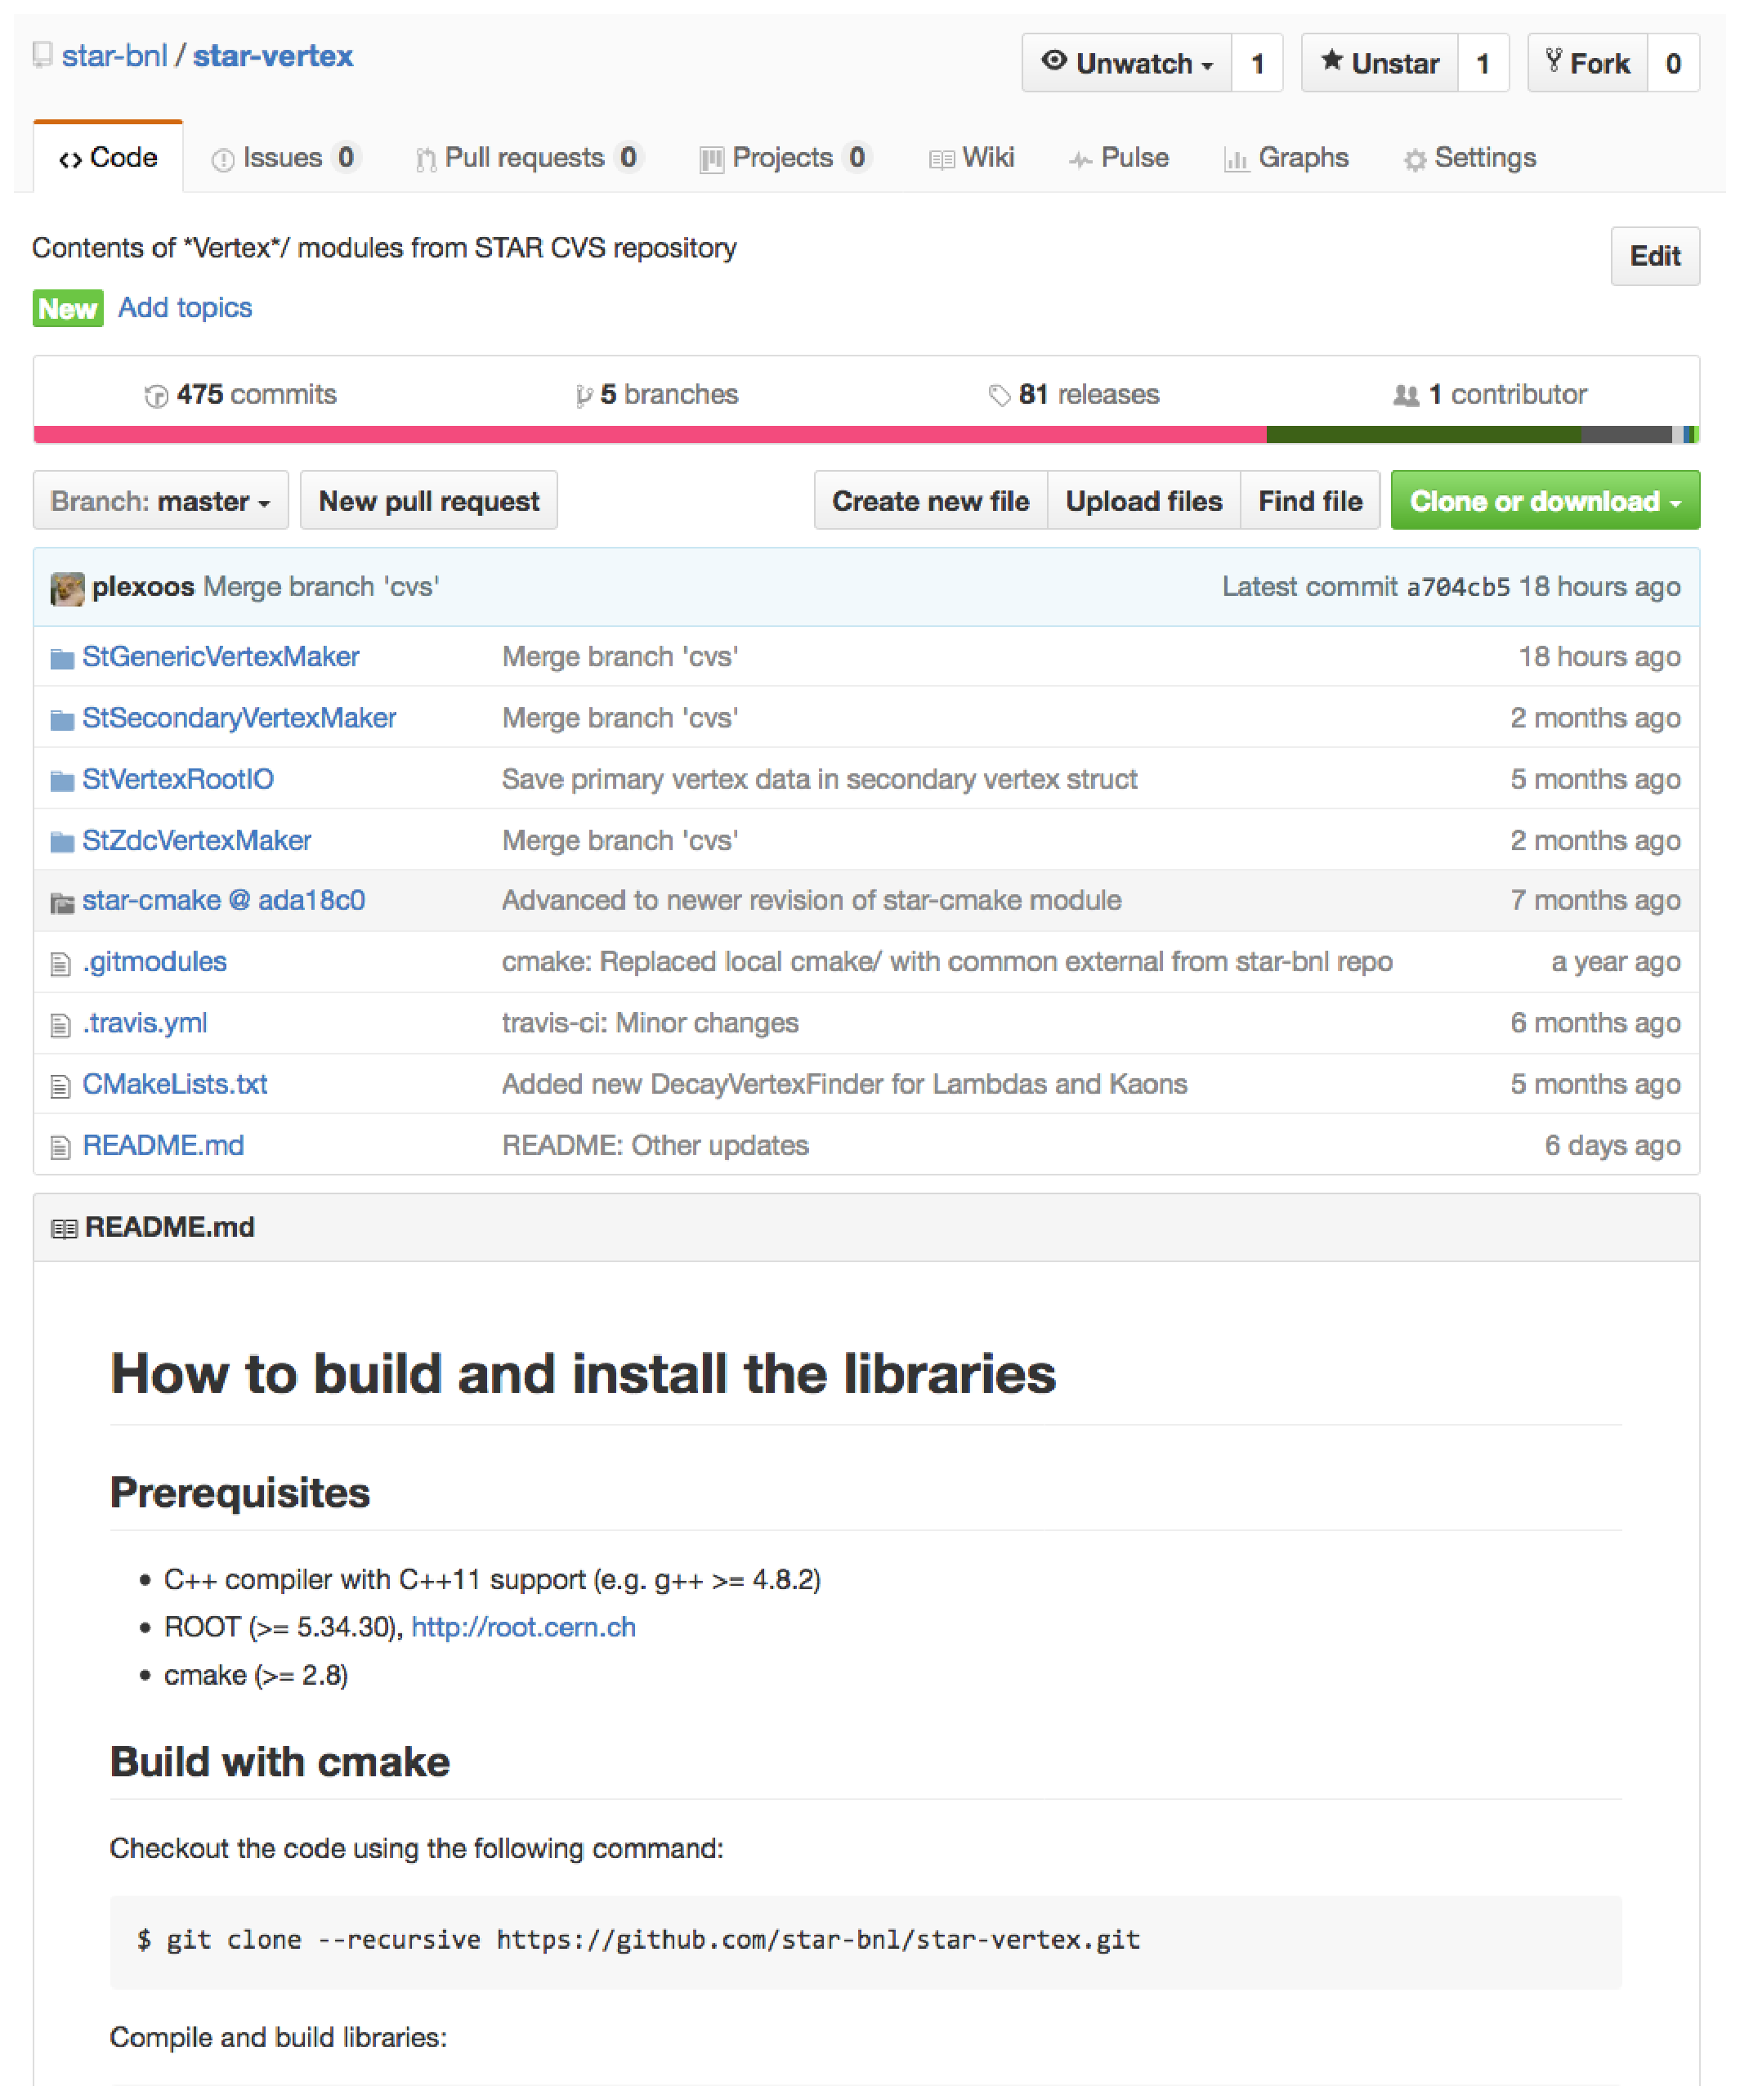
\includegraphics[width=0.45\textwidth]{graphics/github-star-vertex} }


\rput[l](0.0\textwidth, 0.45\textheight) {%
\begin{minipage}{0.50\textwidth}


\raggedright

\begin{list}{\labelitemi}{\setlength{\itemsep}{0mm}
                          \setlength{\topsep}{0mm}}

   \item The source code with instructions/documentation available at\\
   \url{https://github.com/star-bnl/star-vertex}

   \item Periodically synchronized with STAR CVS

\end{list}

\end{minipage}
}



%\psgrid[gridlabels=0.7,subgriddiv=0, griddots=3](1,-1)(0,-3)(\textwidth,\textheight)

\end{pspicture}
%}}}



%===============================================================================
\myfoilhead{-30mm}{Release History: Major Features}
%{{{

\noindent
\begin{pspicture}(0,0)(\textwidth,\textheight)


\rput[t](0.5\textwidth, 0.9\textheight) {%
\begin{minipage}{0.9\textwidth}

\raggedright

\begin{list}{\labelitemi}{\setlength{\itemsep}{0mm}
                          \setlength{\topsep}{0mm}}

   \item Summary of available options for vertex fitting

\end{list}

\quad

\begin{center}
\normalsize

\begin{tabular}{c|c|c|c}

 &
  & \texttt{beamline}
   & \texttt{beamline3D}
    \\
%
 & w/o beamline
  & forced 1D fit
   & 3D fit
    \\ \midrule

\MinuitVF
 & \cmark
  & \cmark
   & \xmark
    \\[3mm]

\PPV
 & \xmark
  & \cmark
   & \xmark
    \\[3mm]

\end{tabular}
\end{center}


\end{minipage}
}


\rput[t](0.5\textwidth, 0.30\textheight) {%
\begin{minipage}{0.9\textwidth}

\raggedright

\begin{list}{\labelitemi}{\setlength{\itemsep}{0mm}
                          \setlength{\topsep}{0mm}}

   \item \textbf{v1.0} --- 2016-03-11

   \begin{list}{\labelitemii}{}

      \item Original code inherited from previous developers
      \item Build with \texttt{cmake}, continuous integration

   \end{list}

\end{list}

\end{minipage}
}



%\psgrid[gridlabels=0.7,subgriddiv=0, griddots=3](1,-1)(0,-3)(\textwidth,\textheight)

\end{pspicture}
%}}}



%===============================================================================
\myfoilhead{-30mm}{Release History: Major Features}
%{{{

\noindent
\begin{pspicture}(0,0)(\textwidth,\textheight)


\rput[t](0.5\textwidth, 0.9\textheight) {%
\begin{minipage}{0.9\textwidth}

\raggedright

\begin{list}{\labelitemi}{\setlength{\itemsep}{0mm}
                          \setlength{\topsep}{0mm}}

   \item Summary of available options for vertex fitting

\end{list}

\quad

\begin{center}
\normalsize

\begin{tabular}{c|c|c|c}

 &
  & \texttt{beamline}
   & \texttt{beamline3D}
    \\
%
 & w/o beamline
  & forced 1D fit
   & 3D fit
    \\ \midrule

\MinuitVF
 & \cmark
  & \cmark
   & \cmark
    \\[3mm]

\PPV
 & \xmark
  & \cmark
   & \cmark
    \\[3mm]

\end{tabular}
\end{center}


\end{minipage}
}


\rput[t](0.5\textwidth, 0.30\textheight) {%
\begin{minipage}{0.9\textwidth}

\raggedright

\begin{list}{\labelitemi}{\setlength{\itemsep}{0mm}
                          \setlength{\topsep}{0mm}}

   \item \textbf{v2.0} --- 2016-12-12

   \begin{list}{\labelitemii}{}

       \item Support 3D vertex fits in \MinuitVF and \PPV
       \item Optional vertex position constraint by the beam line

       \begin{list}{\labelitemiii}{}
          \item Routine to calculate $\chi^2$ for the vertex and the beam line
          \item Proper calculation of uncertainties
       \end{list}
   \end{list}

\end{list}

\end{minipage}
}



%\psgrid[gridlabels=0.7,subgriddiv=0, griddots=3](1,-1)(0,-3)(\textwidth,\textheight)

\end{pspicture}
%}}}



%===============================================================================
\myfoilhead{-30mm}{Release History: Major Features}
%{{{

\noindent
\begin{pspicture}(0,0)(\textwidth,\textheight)


\rput[t](0.5\textwidth, 0.9\textheight) {%
\begin{minipage}{0.9\textwidth}

\raggedright

\begin{list}{\labelitemi}{\setlength{\itemsep}{0mm}
                          \setlength{\topsep}{0mm}}

   \item Summary of available options for vertex fitting

\end{list}

\quad

\begin{center}
\normalsize

\begin{tabular}{c|c|c|c}

 &
  & \texttt{beamline}
   & \texttt{beamline3D}
    \\
%
 & w/o beamline
  & forced 1D fit
   & 3D fit
    \\ \midrule

\MinuitVF
 & \cmark
  & \cmark
   & \cmark
    \\[3mm]

\PPV
 & \cmark
  & \cmark
   & \cmark
    \\[3mm]

\parbox{0.1\textwidth}{\small \centering \PPV\\[-3mm]\&muDST}
 & \cmark
  & \cmark
   & \cmark
    \\[3mm]

\parbox{0.1\textwidth}{\small \centering \MinuitVF\\[-3mm]\&muDST}
% & \textcolor{redDark}{?}
 & \xmark
  & \xmark
   & \xmark
    \\[3mm]

\end{tabular}
\end{center}

\end{minipage}
}


\rput[t](0.5\textwidth, 0.30\textheight) {%
\begin{minipage}{0.9\textwidth}

\raggedright

\begin{list}{\labelitemi}{\setlength{\itemsep}{0mm}
                          \setlength{\topsep}{0mm}}

   \item \textbf{v3.0-rc} --- in progress

   \begin{list}{\labelitemii}{}

      \item Vertex reconstruction using \muDST trees and \PPV vertex finder
      \item Finalize common approach to fitting in \PPV and \MinuitVF
      \item Consolidate track selection in \PPV and \MinuitVF
      \item Unified selection of seeding and fitting algorithms:

      \begin{list}{\labelitemiii}{}
         \item \texttt{SeedFinder: MinuitVF, PPVLikelihood, TSpectrum}
         \item \texttt{VertexFit: NoBeamline, Beamline1D, Beamline3D}
      \end{list}

   \end{list}

\end{list}

\end{minipage}
}



%\psgrid[gridlabels=0.7,subgriddiv=0, griddots=3](1,-1)(0,-3)(\textwidth,\textheight)

\end{pspicture}
%}}}



%===============================================================================
\myfoilhead{-30mm}{Release History: Major Features}
%{{{

\noindent
\begin{pspicture}(0,0)(\textwidth,\textheight)


\rput[t](0.5\textwidth, 0.9\textheight) {%
\begin{minipage}{0.9\textwidth}

\raggedright

\begin{list}{\labelitemi}{\setlength{\itemsep}{0mm}
                          \setlength{\topsep}{0mm}}

   \item Summary of available options for vertex fitting

\end{list}

\quad

\begin{center}
\normalsize

\begin{tabular}{c|c|c|c}

 &
  & \texttt{beamline}
   & \texttt{beamline3D}
    \\
%
 & w/o beamline
  & forced 1D fit
   & 3D fit
    \\ \midrule

\MinuitVF
 & \cmark
  & \cmark
   & \cmark
    \\[3mm]

\PPV
 & \cmark
  & \cmark
   & \cmark
    \\[3mm]

\parbox{0.1\textwidth}{\small \centering \PPV\\[-3mm]\&muDST}
 & \cmark
  & \cmark
   & \cmark
    \\[3mm]

\parbox{0.1\textwidth}{\small \centering \MinuitVF\\[-3mm]\&muDST}
% & \textcolor{redDark}{?}
 & \cmark
  & \cmark
   & \cmark
    \\[3mm]

\end{tabular}
\end{center}

\end{minipage}
}


\rput[t](0.5\textwidth, 0.30\textheight) {%
\begin{minipage}{0.9\textwidth}

\raggedright

\begin{list}{\labelitemi}{\setlength{\itemsep}{0mm}
                          \setlength{\topsep}{0mm}}

   \item \textbf{v3.x} --- planned

   \begin{list}{\labelitemii}{}

      \item Support \muDST-based reconstruction for \MinuitVF

      \item Add primary track association when reconstruct from \muDST

      \item New seed finder based on \texttt{TSpectrum}

      \item Get rid of debugging histograms in production code

      \item \ldots

   \end{list}

\end{list}

\end{minipage}
}



%\psgrid[gridlabels=0.7,subgriddiv=0, griddots=3](1,-1)(0,-3)(\textwidth,\textheight)

\end{pspicture}
%}}}



%===============================================================================
\myfoilhead{-30mm}{Test Samples and Performance Metric}
%{{{

\noindent
\begin{pspicture}(0,0)(\textwidth,\textheight)



\rput(0.50\textwidth,0.45\textheight) {%
\begin{minipage}{0.90\textwidth}

\raggedright

\begin{list}{\labelitemi}{\setlength{\itemsep}{0mm}
                          \setlength{\topsep}{0mm}}

   \item Fully simulated $W$ sample generated with Pythia embedded in Run~13 minbias data\\
   ($pp$ at $\sqrt{s}=510$~GeV)

   \item Vertex reconstruction efficiency is based on known contribution by simulated particles and vertices

   \begin{list}{\labelitemii}{\setlength{\itemsep}{3mm}
                              \setlength{\topsep}{0mm}}

      \item Reconstructed track is matched to a simulated particle by identifying the dominant contributor

   \end{list}

   \item Vertex reconstruction efficiency can be calculated for all vertices or
   only the best match to the simulated one, i.e. the max-rank vertex

   { \centering \rule{0.5\textwidth}{1pt}}

   \item In \muDST reconstruction vertex daughters assigned at final stage

   \begin{list}{\labelitemii}{\setlength{\itemsep}{3mm}
                              \setlength{\topsep}{0mm}}

      \item If track was used in seeding OR $ d/(\sigma_\text{DCA} + \sigma_\text{vertex}) < 1$

      \item Currently assume fully correlated $\sigma_\text{DCA}$ and $\sigma_\text{vertex}$

   \end{list}

\end{list}

\end{minipage}
}



%\psgrid[gridlabels=0.7,subgriddiv=0, griddots=3](1,-1)(0,-3)(\textwidth,\textheight)

\end{pspicture}
%}}}



%===============================================================================
\myfoilhead{-30mm}{\muDST Reco vs. Std Reco}
%{{{

\noindent
\begin{pspicture}(0,0)(\textwidth,\textheight)

\rput[rt](0.5\textwidth,22){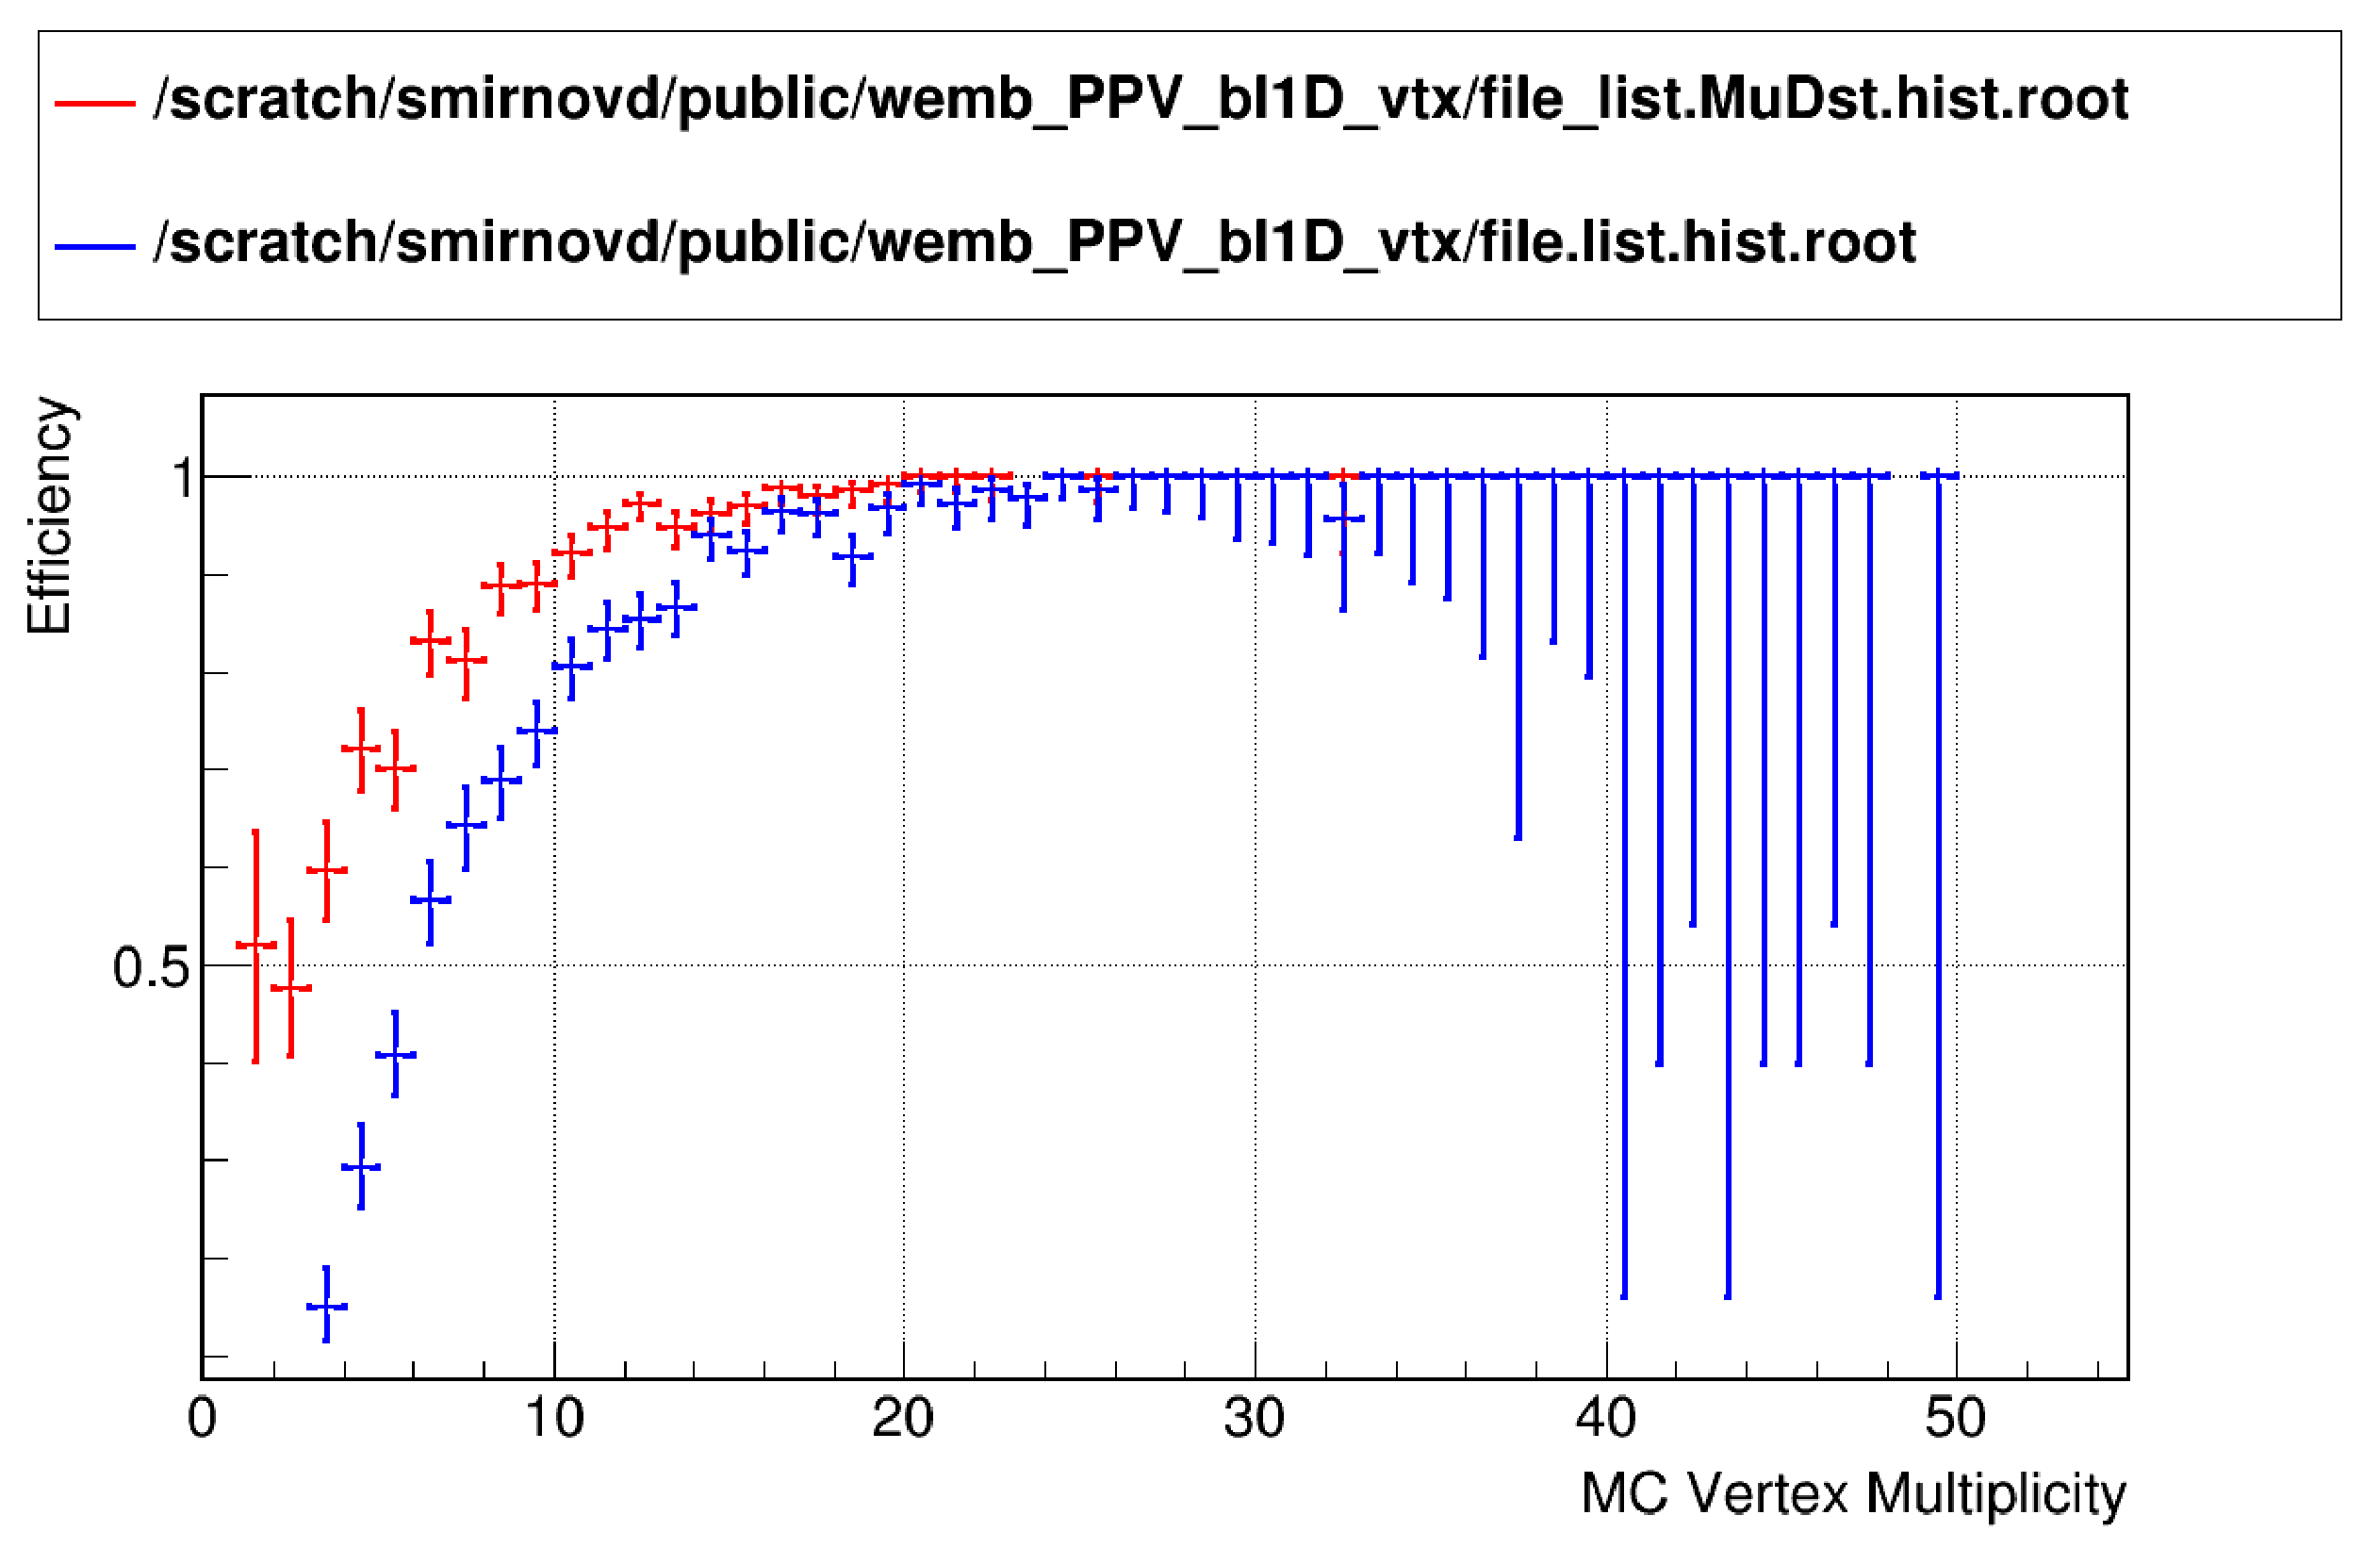
\includegraphics[height=0.5\textheight]{graphics/wemb_PPV_bl1D_muDst_vs_std_reco/event/McRecMulAny_eff}}
\rput[lt](0.5\textwidth,22){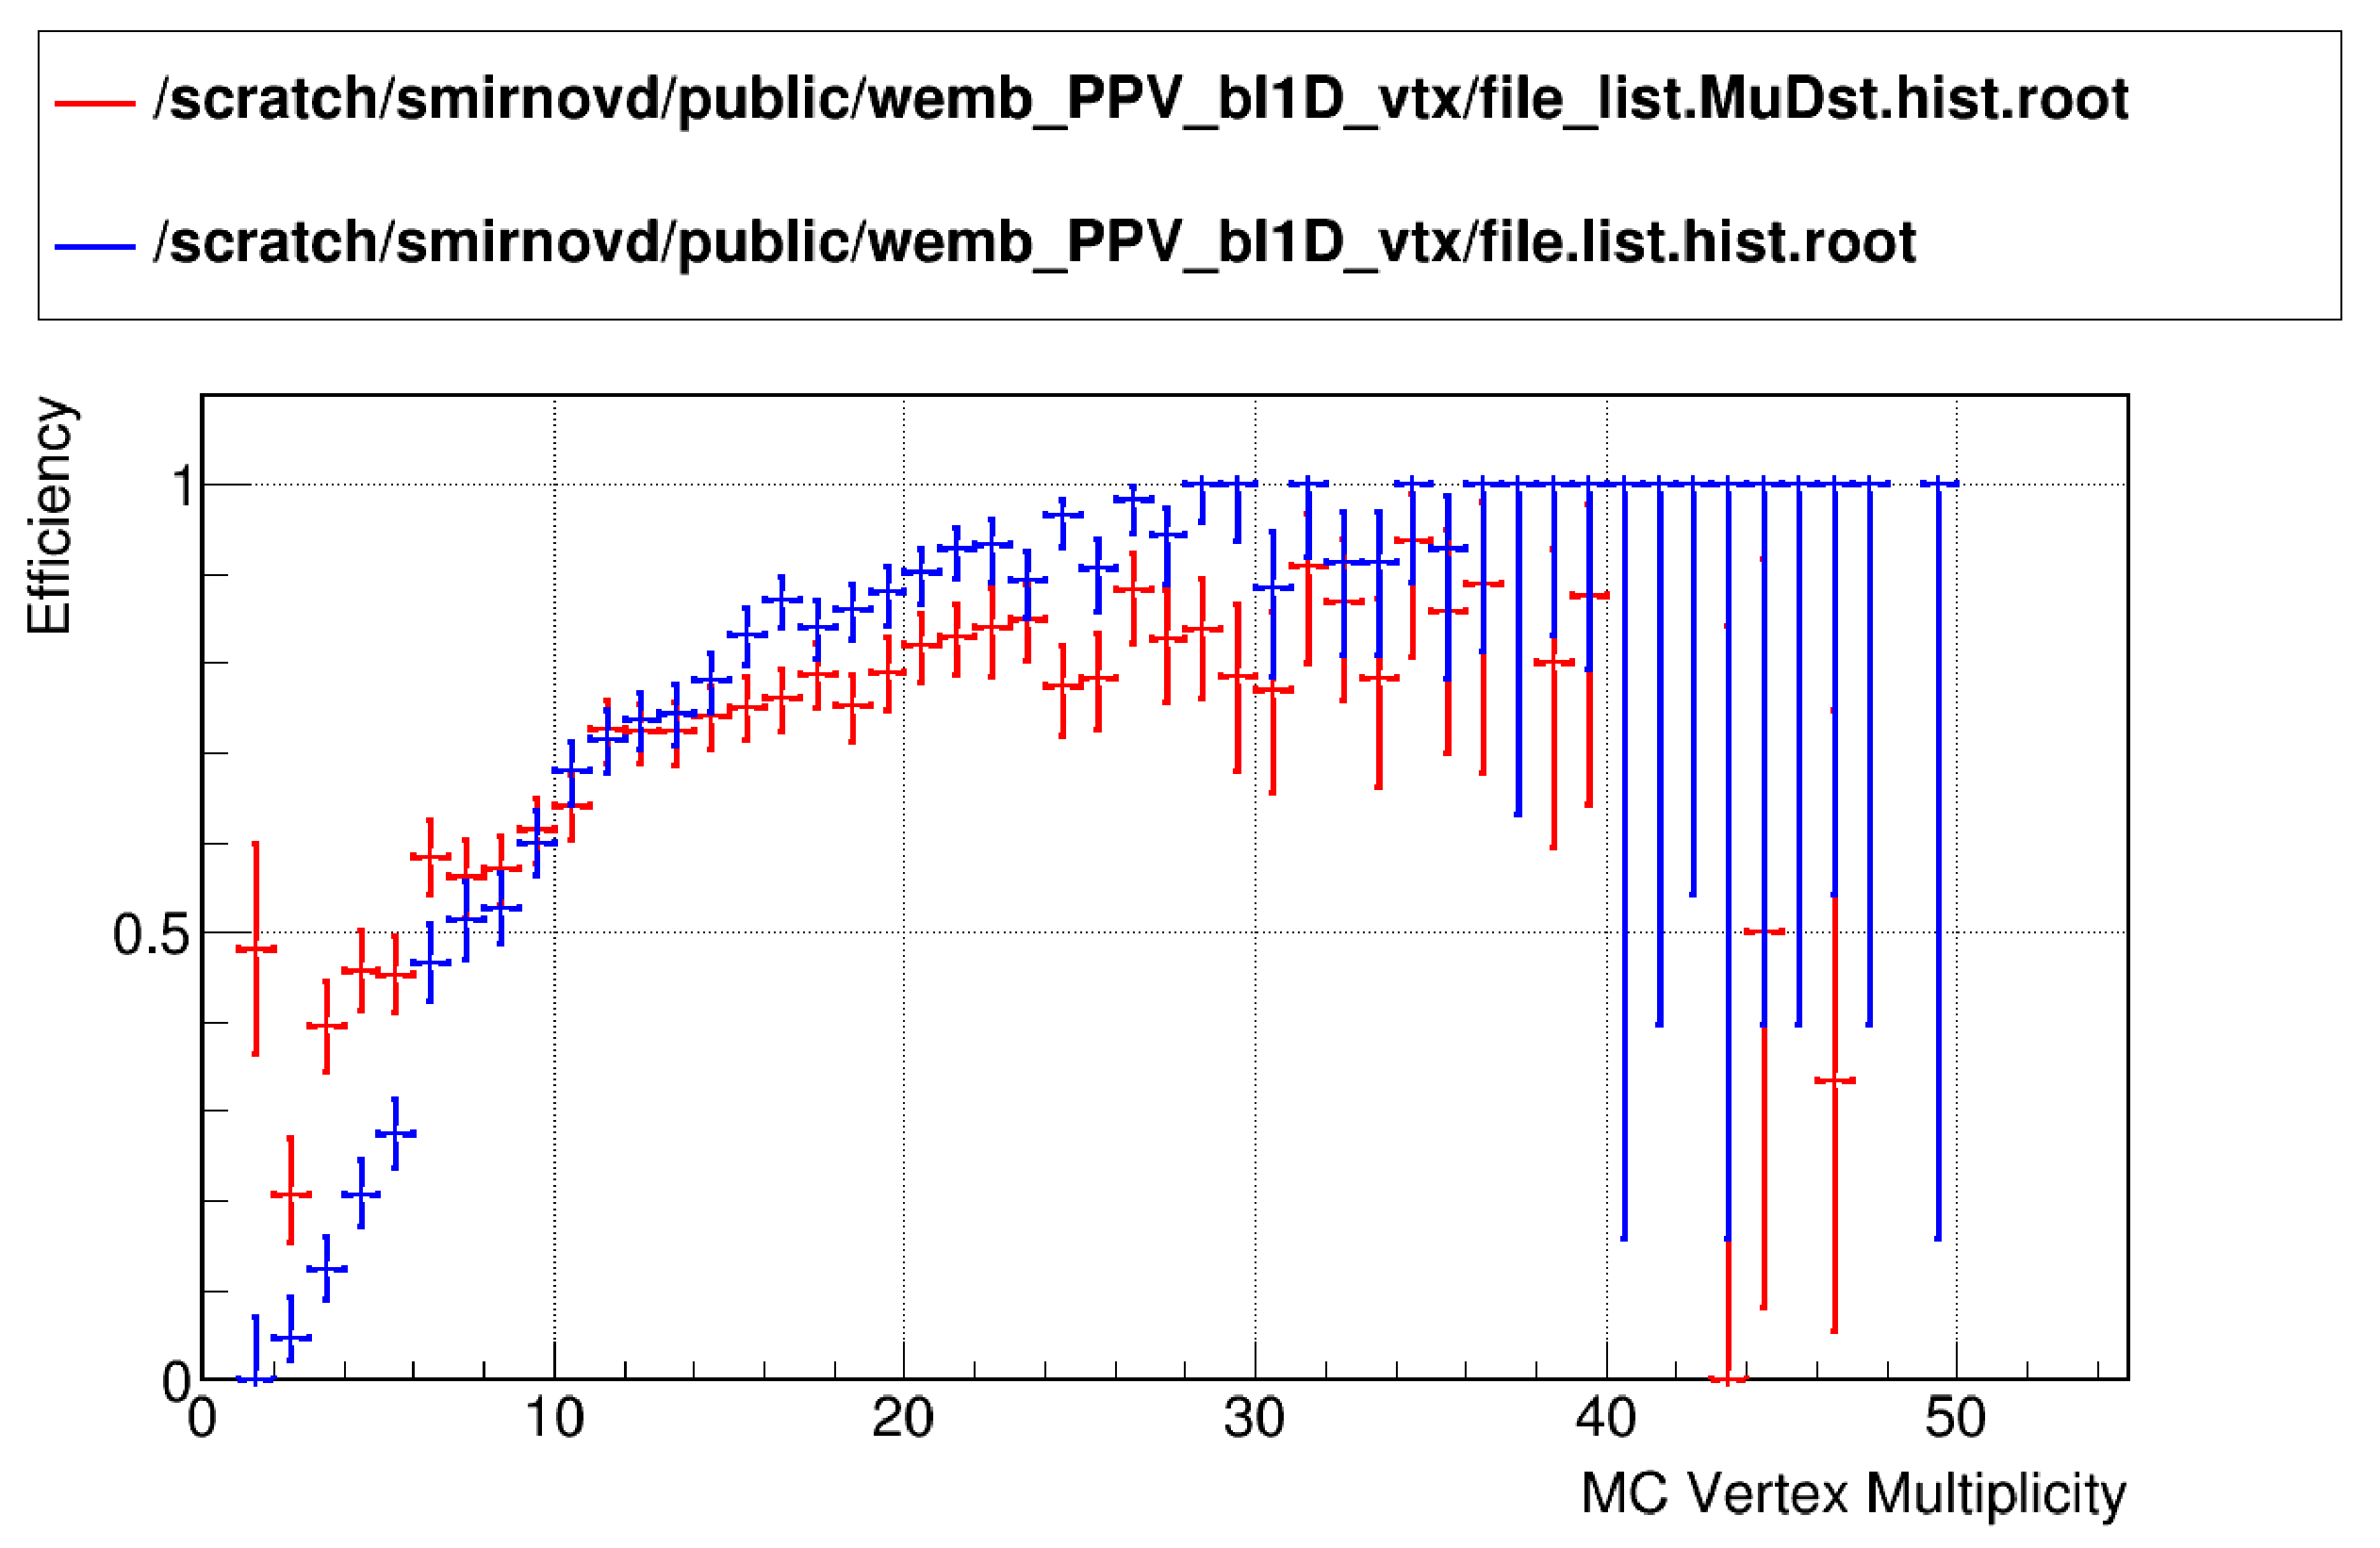
\includegraphics[height=0.5\textheight]{graphics/wemb_PPV_bl1D_muDst_vs_std_reco/event/McRecMulGood_eff}}


\rput(0.5\textwidth, 2) {%
\begin{minipage}{0.90\textwidth}

\raggedright

\begin{list}{\labelitemi}{\setlength{\itemsep}{0mm}
                          \setlength{\topsep}{0mm}}

   \item Unlike with default \Sti-based reconstruction we keep original track-vertex association at seeding stage

   \item This can cause the higher efficiency at low multiplicities

   \item Deficiency for max-rank vertex can arise from non-optimized track-vertex matching criteria

\end{list}

\end{minipage}
}



%\psgrid[gridlabels=0.7,subgriddiv=0, griddots=3](1,-1)(0,-3)(\textwidth,\textheight)

\end{pspicture}
%}}}



%===============================================================================
\myfoilhead{-30mm}{Summary}
%{{{

\noindent
\begin{pspicture}(0,0)(\textwidth,\textheight)



\rput(0.50\textwidth,0.45\textheight) {%
\begin{minipage}{0.90\textwidth}

\raggedright

\begin{list}{\labelitemi}{\setlength{\itemsep}{0mm}
                          \setlength{\topsep}{0mm}}

   \item Proof of concept: Vertices can be reconstructed using \StMuTrack-s

   \begin{list}{\labelitemii}{\setlength{\itemsep}{3mm}
                              \setlength{\topsep}{0mm}}

      \item Speed up factor for VF studies/tuning $\sim 100$'s (no track (re-)reconstruction needed)

      \item Comparable vertex reconstruction efficiency as with \StTrack-s

      \item The code and documentation available $\Longrightarrow$ Can be used by PWG's

   \end{list}

   \item Next

   \begin{list}{\labelitemii}{\setlength{\itemsep}{3mm}
                              \setlength{\topsep}{0mm}}

      \item Investigate different primary track matching methods/cuts

      \item Release v3.0 of STAR vertex libraries. Timescale: $\sim$ one week

      \item Next v3.x release(s) on timescale of $\sim$ one month

   \end{list}

\end{list}

\end{minipage}
}



%\psgrid[gridlabels=0.7,subgriddiv=0, griddots=3](1,-1)(0,-3)(\textwidth,\textheight)

\end{pspicture}
%}}}



%===============================================================================
\label{slide:last}

\end{document}
